
\documentclass[12pt,dvipsnames]{exam}
\usepackage[utf8]{inputenc}
\usepackage[colorlinks=true, urlcolor=blue]{hyperref}
\usepackage[spanish]{babel}
\usepackage{graphicx}
\usepackage{amsmath}

\begin{document}

\title{Cuaderno de Laboratorio - Tesis}
\author{JRR (10) and H. G. + LEC}
\maketitle






$17/9/2019$

Corrida del barrido tomó 44.18 minutos.

$dx = dy = 100$ micrones ó $0$.$1$ mm


\hrulefill


$21/9/2019$

CITA del siguiente \href{https://www.iridian.ca/technical-resources/articles-whitepapers/eyes-skies-optical-filters-earth-observation/}{link}:

\url{https://www.iridian.ca/technical-resources/articles-whitepapers/eyes-skies-optical-filters-earth-observation/}

\textit{However, observation from orbit has presented its own set of challenges and associated solutions:}

\begin{itemize}
\item CHALLENGE 1: see through the atmosphere (clouds/aerosols) or in some cases observe only these atmospheric constituents or phenomena
\item SOLUTION 1: wavelength selective imaging
\item CHALLENGE 2: observe small signals in a large background scene
\item SOLUTION 2: large, highly uniform collection optics
\item CHALLENGE 3: pack as much measurement capability into as small and lightweight a package as possible to reduce launch costs
\item SOLUTION 3: compact/multi-spectral imaging
\item CHALLENGE 4: determine the type of phenomena (“what”) and location (“where”) under observation from a distance (eg. low earth orbit is 160-2000 km above the earth’s surface)
\item SOLUTION 4: combination of high spatial (“where”) and spectral (“what”) resolution
\item CHALLENGE 5: survive launch conditions and operate outside of earth’s protective atmospheric blanket
\item SOLUTION 5: robust and reliable optical components
\end{itemize}

FIN cita. Se observa que cada item de los de arriba podría ser un aspecto técnico del futuro \textsc{datasheet}.


Con respecto al challenge 2 cuya solución es \textit{Large, Highly Uniform Collection Optics}, se encontró en la página del fabricante \textsc{Iridian}, un gráfico similar al que se quiere reproducir con el barrido espacio-espectral del filtro: 

\begin{center}
	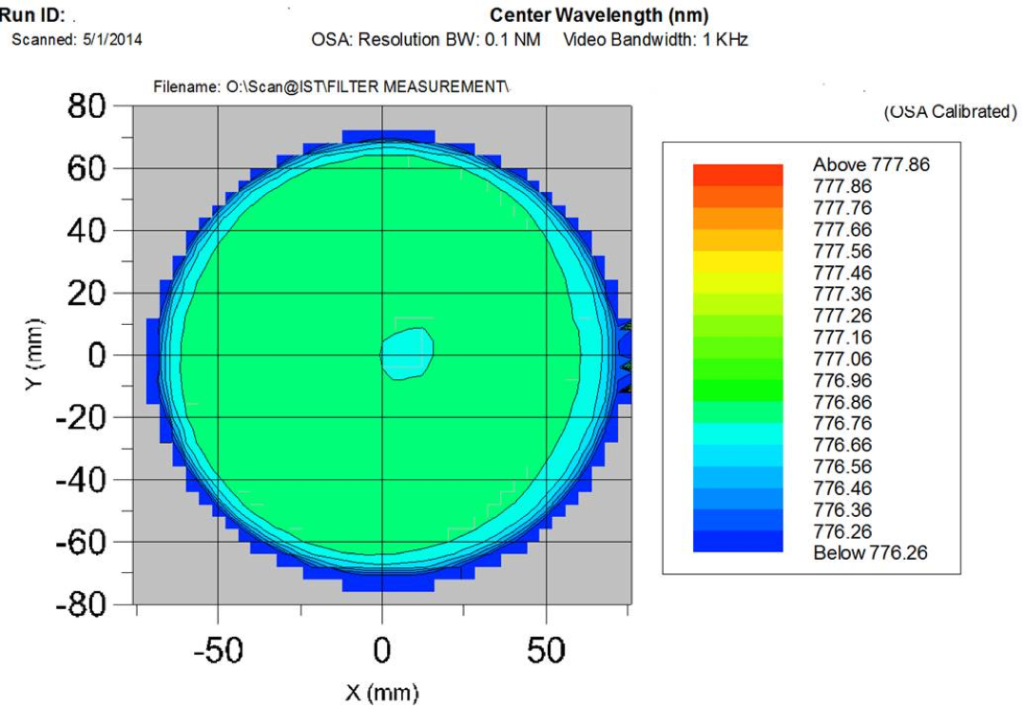
\includegraphics[scale=1.0]{imgs/barr_iridian.png}
\end{center}


De las mediciones del $17/9$, la banda verde tiene el siguiente espectro, parece ser bastante homogénea la banda, es decir que en cada punto x,y espacial de la banda el espectro de transmisión parece ser el mismo (esto habría que confirmarlo), se puede caracterizar con algún parámetro la homogeneidad del filtro? $\xrightarrow{}$ El objetivo de esta parte es lograr una buena \textsc{datasheet} del filtro.

\begin{center}
	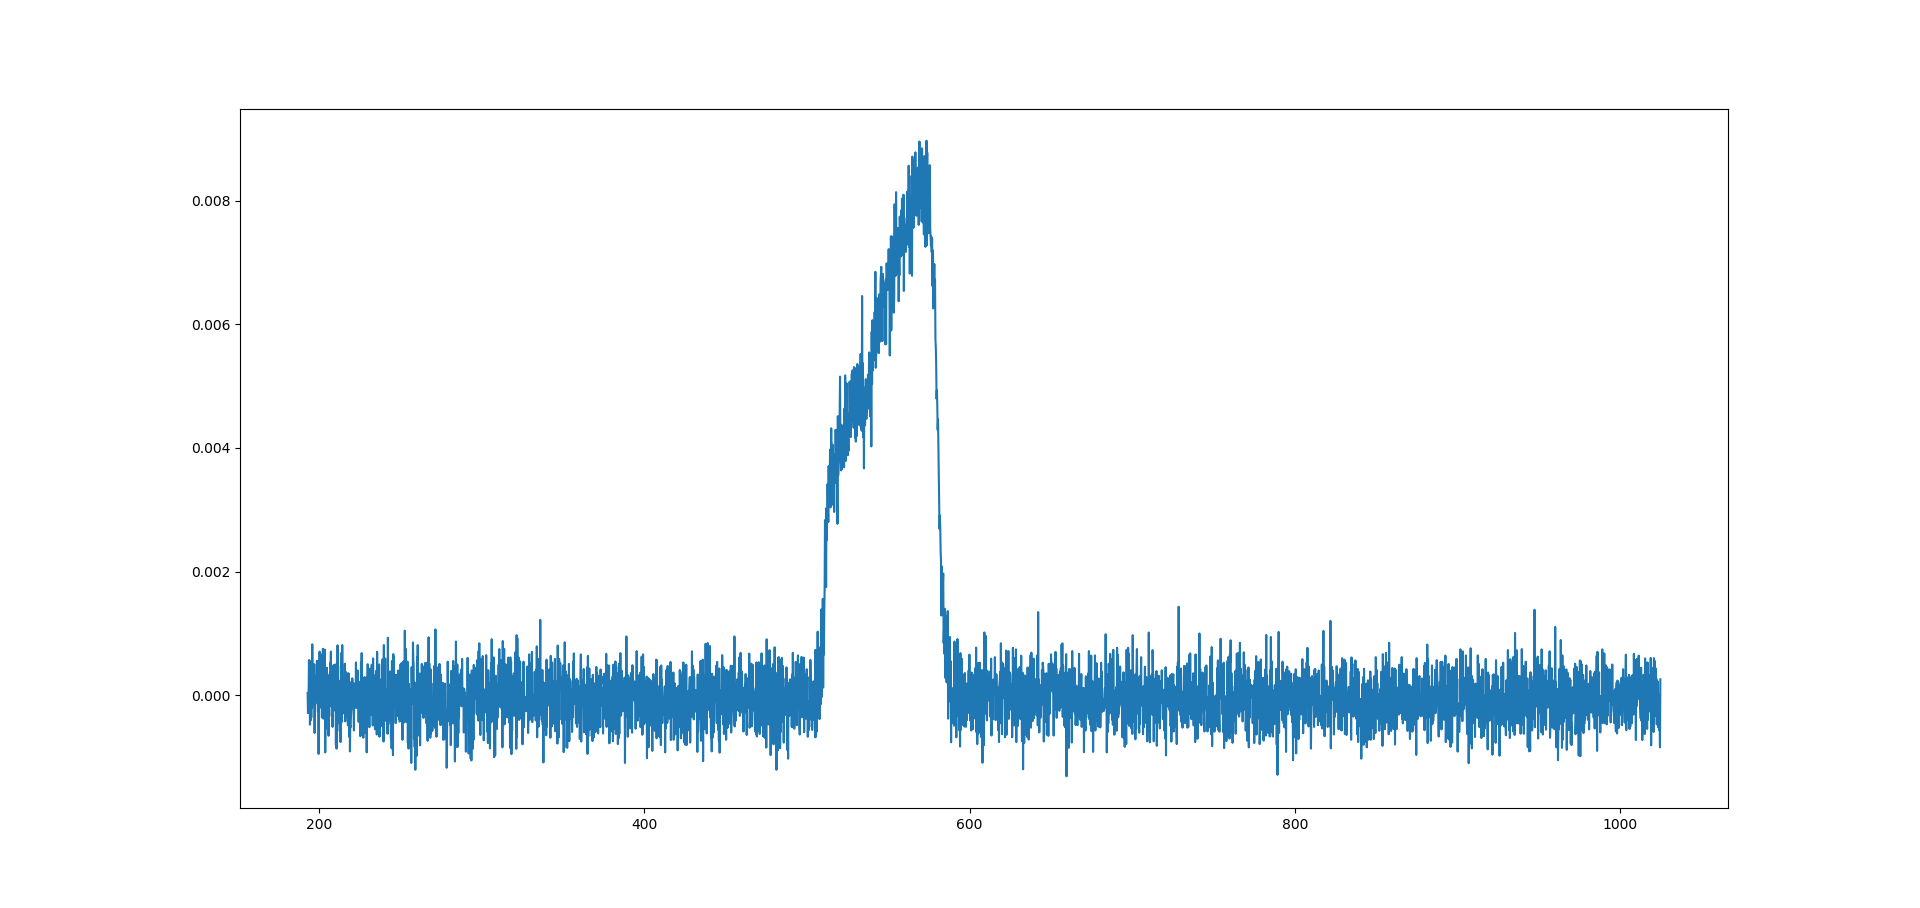
\includegraphics[scale=0.4]{imgs/green_band_spectra.png}
\end{center}


Ejemplo de datasheet del fabricante \textsc{Iridian}, sacado de \href{https://www.iridian.ca/product/bpf-9460-180/}{aquí}:

\begin{center}
	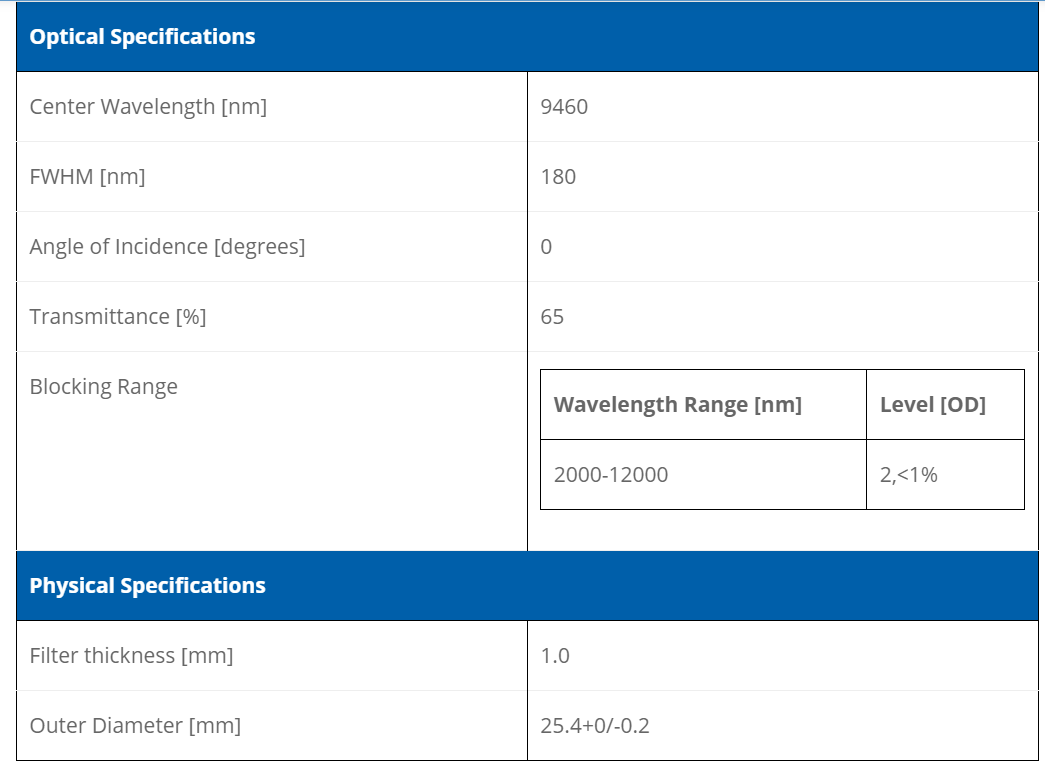
\includegraphics[scale=1.0]{imgs/datasheet_modelo.png}
\end{center}


\end{document}
